
%\vspace{-0.4cm}
\section*{Model}
\vspace{-0.2cm}

Motivated from the observed anisotropy in axonal morphology (Fig.~\ref{fig:morphaniso}) we formulate an \textit{anisotropic network model}: $N=1000$ neurons are distributed uniformly on a square of length \SI{296}{\micro\meter}. Each neuron is assigned a random direction $\alpha \in [0,2\pi)$ and connections are established to target neurons lying within in a corridor of width $w=\text{\SI{74.6}{\micro\meter}}$ (Fig.~\ref{fig:4nets}). Here $w$ was tuned to obtain a network connection density of $p=11.6$ as found in \cite{Song2005}.

\begin{center}\vspace{0.01cm}
  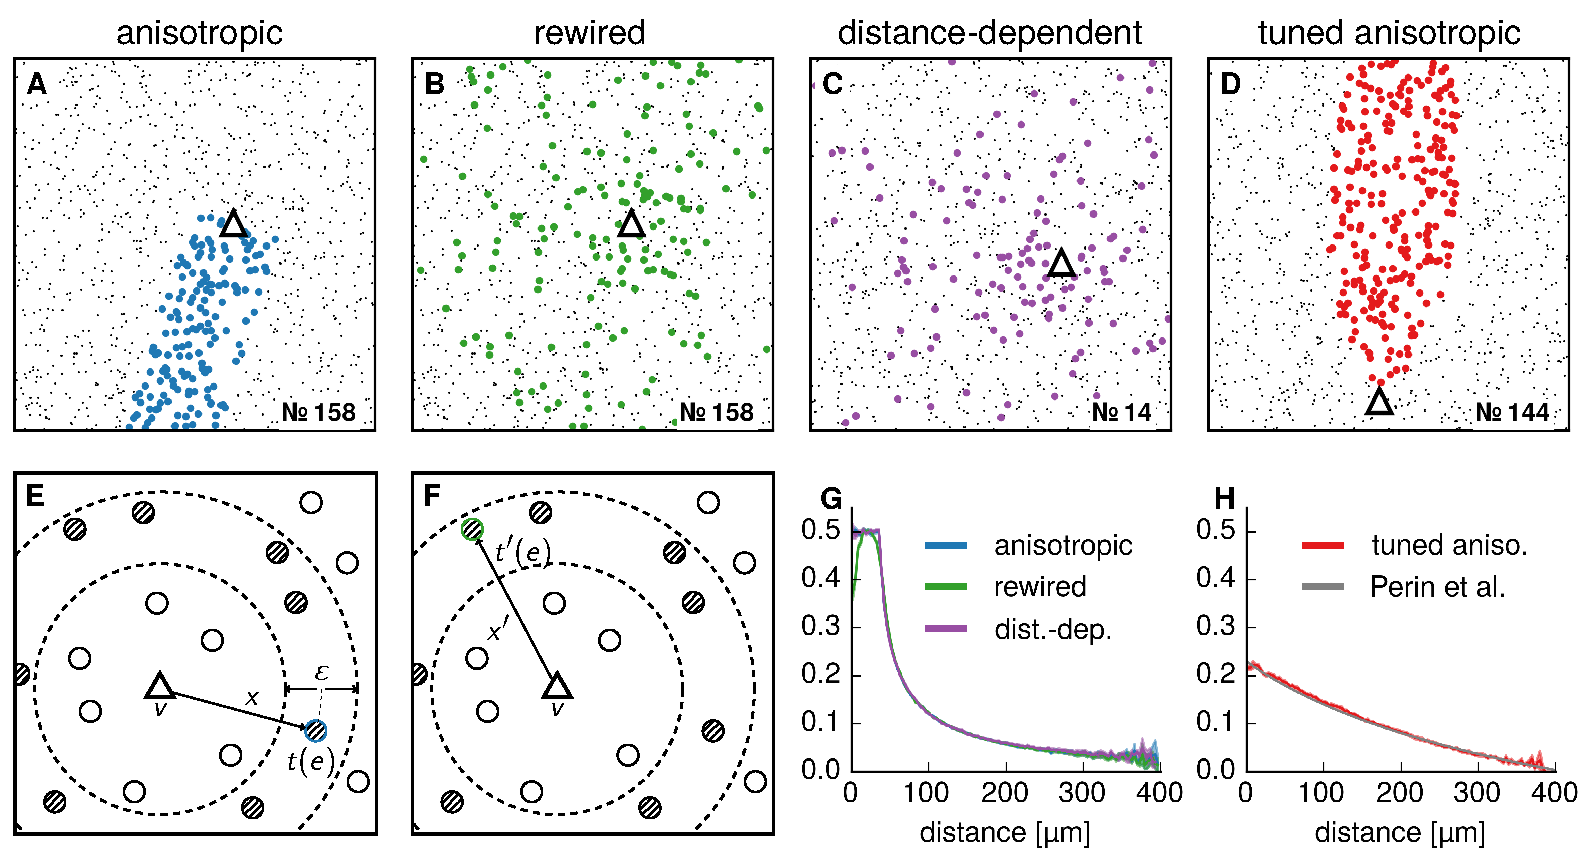
\includegraphics[width=\columnwidth]{%
    /home/fh/sci/rsc/aniso_netw/pub/arxiv18/figures/4_network_models/4_network_models.pdf}
  \captionof{figure}{Spike-timing dependent plasticity changes synaptic efficacies additively, while synaptic normalization acts multiplicatively on the synaptic weights.}
  \label{fig:4nets}
\end{center}\vspace{2cm}




